\documentclass[a4paper,10pt]{article}
\usepackage[margin=2.5cm]{geometry}
\usepackage[utf8]{inputenc}
\usepackage[colorlinks=true,urlcolor=blue]{hyperref}
\usepackage{amsmath}
\usepackage{graphicx}
\usepackage{float}
\usepackage{caption}
\usepackage{subcaption}
\usepackage{minted}



\setlength{\parindent}{0em}
\setlength{\parskip}{1em}

\begin{document}
\begin{titlepage}
    \centering
    \vspace*{2cm}
    {\Huge \textbf{1RT730 Project Report} \par}
    \vspace{0.5cm}
    {\LARGE Harald - Your Personal Chat-Powered Language Partner \par}
    
    \vspace{2cm}
    
\includegraphics[width=0.6\textwidth]{cute_thinking_harald.png} % your image
    \vspace{2cm}
    
    {\Large Joel Sundin, Petter Möllerström, Rahul Sebastian Peter \par}
    \vspace{1cm}
    {\large \today \par}
\end{titlepage}   
\newpage

 \section{Introduction}
Learning Swedish as a non-native speaker presents significant challenges, particularly when opportunities for interactive practice and real-time feedback are limited. To address these challenges, this work proposes \textit{Harald}, an AI-driven language learning application that leverages Large Language Models (LLMs), quizzes, and flashcard functionalities to enhance engagement and personalization in language acquisition.

Harald integrates multiple learning modalities to support comprehension, vocabulary retention, and conversational skills. Beyond individual learning, Harald contributes to societal language inclusivity by supporting immigrants, students, and professionals in their integration into Swedish society. The primary contribution of this study lies in the integration of LLM-based interaction within a structured learning framework, enabling personalized practice, targeted feedback, and contextual understanding in a scalable and accessible manner.

Harald is implemented as a web-based application, allowing learners to access its features directly through a standard browser without the need for local installation. This design choice enhances accessibility and convenience, enabling learners to practice Swedish anytime and anywhere, whether on desktop or mobile devices. By combining cloud-based LLM computation with an intuitive browser interface, Harald ensures that advanced language processing capabilities are delivered seamlessly to users, while maintaining a lightweight and user-friendly experience.

The system’s web-based nature also facilitates easy updates and integration of new exercises or models, ensuring that learners always benefit from the latest functionality Harald has to offer. Overall, Harald provides a comprehensive, adaptive, and accessible environment for Swedish language learning, bridging the gap between traditional pedagogical methods and modern AI-assisted instruction.

\section{Dataset}

The development of the Swedish language tutoring chatbot involved several iterations of dataset design and experimentation aimed at improving the model’s performance, naturalness, and pedagogical value. Over the course of the project, multiple datasets were constructed and evaluated, ranging from community-sourced linguistic discussions to synthetically generated dialogue data. Ultimately, however, the final system adopted a different strategy that relied on prompt engineering and curated conversational examples rather than direct fine-tuning. The main dataset iterations are described below.

\subsection{Reddit-based corpus}
The initial dataset was collected from the r/swedish subreddit using the Python Reddit API Wrapper (PRAW). This community consists of users interested in learning or discussing the Swedish language, and thus provides an organic dataset composed of learner questions and native or advanced speaker responses. The dataset comprised approximately 6,500 comments, each representing short-form discussions about grammar, vocabulary, pronunciation, and translation. Preliminary fine-tuning experiments were conducted using this dataset to adapt a general-purpose language model to the linguistic style and content of Swedish language learners. However, despite its relevance, the dataset exhibited several limitations, including inconsistent quality, informal tone, and limited conversational depth. Consequently, it was deemed insufficient as a primary fine-tuning source.

\subsection{Synthetic dialogue dataset}
In the second iteration, a manually constructed dataset of user–assistant interactions was developed to simulate tutoring dialogues. These pairs were designed to represent common learner scenarios such as vocabulary practice, grammar correction, and cultural explanations. This dataset was later expanded using generative augmentation, where additional examples were synthesized with Anthropic’s Claude Sonnet model. The resulting dataset provided higher-quality, domain-specific examples and was used for initial LoRA-based fine-tuning experiments. While the synthetic data improved linguistic consistency, further evaluation revealed limited benefits relative to the computational cost of model adaptation.

\subsection{Web-scraped Swedish news dataset}
To provide learners with authentic, up-to-date material for reading comprehension and writing practice, a web scraper was implemented to collect recent Swedish news articles from online media outlets. The system allows users to choose from a selection of articles and engage in follow-up exercises such as summarization or open-ended question answering. This component operates dynamically at runtime rather than as part of the fine-tuning dataset, ensuring continuous exposure to contemporary language usage and diverse topics.

\subsection{Flashcard-based vocabulary dataset}
An auxiliary feature enables users to store specific words encountered during interaction into a personal flashcard list for later review. Although not a dataset in the traditional training sense, this mechanism contributes to personalized learning and vocabulary retention through spaced repetition.

\subsection{Final data strategy}
In the final system, neither the Reddit corpus nor the synthetic fine-tuning datasets were employed in the deployed model. Instead, the chatbot is based on a fully pretrained large language model (Gemini 2.5 Flash), with its pedagogical behavior governed by an extensive system prompt. This prompt defines the tutor’s persona, instructional goals, and tone, supplemented by curated example dialogues that demonstrate effective interaction patterns. This approach provided greater flexibility, reduced training costs, and preserved the model’s general linguistic competence while enabling targeted guidance for Swedish language tutoring.

\section{Architecture}
The overall design of the application follows a modular, multi-page architecture implemented in \texttt{Streamlit}, with each functional page focusing on a distinct aspect of language learning. The system integrates Google’s \textbf{Gemini 2.5 Flash} model as its core language engine and uses \texttt{Streamlit’s session state} as a lightweight internal memory layer to maintain user progress and contextual continuity across pages.

The entry point of the application is a simple landing page that serves primarily as a user gateway, providing a clean introduction to the application/website without incorporating functional logic. From this page, the user navigates to the four core learning environments: the \textit{Chat}, \textit{Quiz}, \textit{Comprehension}, and \textit{Flashcards} pages. Each of these modules operates independently in terms of interface, yet the Quiz, Chat and Flashcard pages share a common backend design and a unified state through the \texttt{session\_state} object, ensuring that progress and user data persist as the learner moves between pages.

The \textit{Chat page} represents the primary conversational interface where the user interacts directly with the language model, \textit{“Harald”}. Upon initialization, the system dynamically constructs a comprehensive system prompt combining Harald’s pedagogical persona, presents the model with a variety of example conversation snippets along with contextual data about the learner’s recent performance. If the user has completed a vocabulary quiz, the prompt automatically includes their score, the number of questions answered, and a list of incorrectly answered items. This personalized prompt is then passed to the Gemini model via the Google Generative AI API, ensuring that each dialogue session is pedagogically adaptive. The user’s messages and the model’s replies are appended to the conversation history, which is persistently stored in both the session memory and a JSON file for continuity between visits. 

The \textit{Quiz page} implements a randomized multiple-choice test drawn from a pre-defined dataset of Swedish vocabulary terms. The system tracks the user´s responses, calculates the total score, identifies incorrectly answered items, and updates the highest score if applicable. This data is saved in the session state and becomes part of the learner’s context on the chat page, allowing Harald to provide individualized tutoring that directly addresses the learner’s weaknesses. This design choice creates a feedback loop between assessment and instruction, supporting the application’s pedagogical goal of adaptive reinforcement.

The \textit{Comprehension page} is meant to assess the user´s comprehension and writing. It selects a short Swedish article from a predefined dataset and offers two distinct modes: summarization or comprehension questions. In summarization mode, the user writes a short summary in Swedish, which is then evaluated by the LLM using a system prompt designed to generate constructive feedback, grammar corrections, and stylistic suggestions. In comprehension mode, the model first generates a small set of reading comprehension questions in Swedish, after which the user answers them manually. The model then evaluates the responses and provides individualized feedback in a supportive tone. 

The \textit{Flashcards page} serves as a lightweight review module, reinforcing vocabulary encountered during chats or quizzes. Flashcards are created automatically when the user or the model triggers the “add flashcard” tool during conversation. Each flashcard includes a Swedish term, its English translation, and metadata describing its origin (e.g., from chat or quiz). When revisiting the flashcard page, the user can randomly select a card, attempt to recall its meaning, and receive immediate corrective feedback. The simplicity of this interaction supports microlearning and vocabulary retention.

From a system perspective, all components are unified by the underlying LLM integration pattern. The application interfaces with Gemini through a \texttt{genai.Client} instance, configured with \texttt{GenerateContentConfig} objects that define system prompts, temperature settings, and tool availability. This modular prompt-building approach allows each page to construct specialized prompts suitable for its learning context (conversation, evaluation, summarization, etc.), while maintaining a consistent personality and tone, ensuring pedagogical consistency while allowing for functional diversity.

The architectural design  in this project follows three key principles. First, \textit{context persistence}: the session state mechanism ensures that user data, learning history, and model context are retained across activities. Second, \textit{modular extensibility}: each learning component (chat, quiz, comprehension, flashcards) is implemented as an independent Streamlit page, making it straightforward to modify or extend functionality without affecting other modules. Third, \textit{adaptive personalization}: by feeding user performance data directly into the system prompts, the model dynamically adjusts its responses and focus areas to align with the learner’s evolving needs. Together, these principles enable a seamless integration of assessment, interaction, and reinforcement—transforming the LLM from a passive conversational agent into an active and context-aware tutor.

\section{Results}

\subsection{Quantitative analysis}

To quantitatively analyze the accuracy and correctness of the responses generated by Harald, a list of 100 questions related to Swedish words and grammar were created. We fed these questions to Harald one at a time to generate a response. The responses were then manually checked for correctness. A four-valued scale was used to label each response:

\begin{itemize}
    \item \textbf{Correct}: the response was correct and complete.
    \item \textbf{Incomplete}: the response was correct, but missed some important details, such as verb gender.
    \item \textbf{Partially incorrect}: the response contained some inaccurate information, such as grammar errors in examples.
    \item \textbf{Incorrect}: the response contained mostly or only incorrect information.
\end{itemize}

\begin{figure}[htbp]
    \centering
    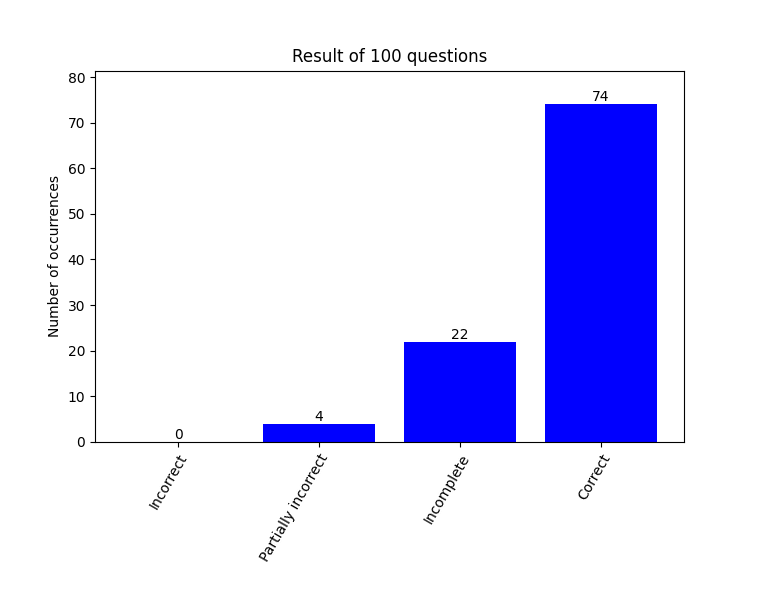
\includegraphics[width=0.8\linewidth]{quant_results.png} % adjust width as needed
    \caption{Bar chart showing the quantified accuracy scores.}
    \label{fig:quant_results}
\end{figure}

Figure \ref{fig:quant_results} shows the results of the evaluation. As can be seen from the chart, the responses were correct and complete 74\% of the time, and partially incorrect 4\% of the time. None of the responses were mostly or fully incorrect. 

\subsection{Qualitative Analysis}

To understand how users experienced the chatbot we shared it with several participants and collected their feedback using a Google Form. The participants included from people who have no proficiency in Swedish to people who have intermediate proficiency. The form included questions about usability, personalization and learning experience. Most of the feedback received was positive showing that users found the chatbot engaging and helpful for practicing Swedish reading and writing. Many participants mentioned that they would use it again or recommend it to others.

When asked \textit{“What kind of improvements would make the chatbot feel more personalized to you?”}, a common suggestion was that the chatbot could ask more questions about the user at the beginning or check their current knowledge level. This would help adapt the responses and examples to each user’s background and learning pace.

In response to \textit{“What did you dislike or find confusing?”}, one participant mentioned that the reading texts felt too difficult for their level. This feedback highlights a limitation of the current version that it does not adjust the difficulty of reading materials based on the learner’s proficiency.

Overall the qualitative feedback suggests that users appreciated the chatbot’s friendly tone and learning support but would like more personalization and difficulty adaptation in future versions. These insights will guide further development to make the chatbot more engaging and effective for learners at different stages in their learning.

\section{Societal Impact}
The use of large language models (such as Gemini 2.5 Flash) has a strong influence on society. These models can bring many benefits but also create new challenges that must be handled responsibly.

\subsection{Positive Implications}
The main benefit of Harald is improved accessibility and inclusion. Learners from different backgrounds can practice Swedish anytime without the need for expensive language courses or native-speaking tutors. This can support immigrants, students and professionals who want to integrate into Swedish society more easily. The chatbot also improves educational efficiency offering instant corrections, feedback and explanations in simple English. It encourages personalized learning allowing users to progress at their own pace and supports the democratization of knowledge by making language learning resources available to a wider audience.

\subsection{Negative Implications}
However, there are several potential risks to be addressed. Since Harald uses the Gemini model, it relies on a pre-trained dataset that we do not have any control over. This means potential biases, inaccuracies or cultural insensitivities from the training data can surface in responses. The only adjustable parameter is the system prompt, which helps guide the model’s tone and focus but it might not be effective in all edge cases. There are also parameters which restrict harmful and hateful dialogues but inspite of all these techniques it is difficult to guarantee perfect accuracy or fairness in all interactions. There are also privacy concerns because users might share personal details in their messages. This requires careful data handling and protection. Another risk is that users could become too dependent on the chatbot or overconfident on AI-generated responses and use it instead of real conversations with people. In addition using large models like Gemini has an environmental cost, since it requires high energy use for both training and running the model.

\subsection{Ethical Considerations and Mitigation}
To manage these issues the system should be transparent about being an AI and not a real teacher. Users should understand that it may not always be correct or unbiased. The system prompts should be regularly updated to make the responses more reliable and human reviews can help check for mistakes or bias. Personal information should be anonymized or removed and data storage should follow privacy regulations. Using smaller or optimized versions of the model can also help lower the environmental impact.

While Harald highlights the educational and social benefits of integrating LLMs into language learning, ongoing monitoring is essential. Balancing accessibility and personalization with fairness, accuracy and ethical responsibility will determine the long-term success and trustworthiness of such systems in society.
	
\hfill \break
\textit{\textbf{Use of generative AI}}

Generative AI was used for formatting the text for writing this report. It was also used to create example chatbot conversation to use as system prompts for making the chatbot accessible and personlized.


\hfill \break


\begin{thebibliography}{1}

\bibitem{google_gemini}
Google AI. \textit{Gemini API Text Generation Documentation.} 
Available at: \url{https://ai.google.dev/gemini-api/docs/text-generation}

\bibitem{gemini_functions}
Google AI. \textit{Function calling with the Gemini API.} Available at: \url{https://ai.google.dev/gemini-api/docs/function-calling}

\end{thebibliography}


	
	
%	\pagebreak
%	
%	\appendix
%	\section{Code}
%	\label{app:code}
%	
%	\inputminted[frame=lines,framesep=2mm,linenos]{python}{your_code.py}
%	
\end{document}
